\section{Conclusion}
In this chapter, we have identified two mechanisms to get a global representation of a heterogeneous system: \emph{composition} and \emph{coordination}. 

We have presented approaches that compose heterogeneous models/languages to obtain a new model/language. The composition of models has been automated by looking for correspondences between heterogeneous models, and then composing them into a new model that conform to another language. While most of the approaches only consider structural correspondences, only few consider also the behavior of models to find similarities. Furthermore, we have determined that these approaches only compose homogeneous models. This limits the use of such approaches in complex systems where heterogeneous behavioral models may be used. 

We have presented approaches that compose languages to get a new language. Most of these approaches focus on the composition of the syntax of languages into a new syntax. Only Semantics Anchoring~\cite{semanticsanchoring} proposes to compose behavioral semantics by relying on the notion of Semantic Units. These approaches propose to model a heterogeneous system by relying on a single language which results from the composition of other languages. From our point of view, language composition approaches are not suitable for separation of preoccupations and development of a single system by various domain experts who focus on a specific part of the system.

We have presented state-of-the-art approaches that deal with coordination of the behavior of heterogeneous models/languages. First, we have presented the work done by Coordination Languages and ADLs that support the coordination of heterogeneous models. However, the system designer has to manually specify each relation, thus making this task tedious and error prone. Then, we have shown how language coordination approaches have leveraged on the know-how of system designer to automate the coordination between models. However, we have noted that the knowledge about system integration is encoded within a framework. Furthermore, in frameworks, the model of coordination is expressed by using a general purpose language thus limiting verification and validation activities. 

In this thesis, we rely on the coordination of (heterogeneous) behavioral models to get the emerging system behavior of a heterogeneous system. We propose to automate the coordination between models by specifying coordination patterns between languages. Such a pattern leverage on the know-how of a system designer. To specify coordination patterns, a language integrator should rely on a dedicated language as in the case of model composition approaches. Such specification defined at language level should enable a system designer to synthesis a coordination model when applied between particular models. The generated model of coordination should be expressed in a formal language to enable reasoning on the global system. 

In the next chapter, we elaborate on these requirements and we present a framework for the specification of coordination patterns. From these requirements, we propose a language for capturing the specification of coordination patterns named \bcool. Then, in chapter~\ref{ch:bcool}, we present the implementation of our language.





%We want to highligne that the current integration of languages is based on two mechanism: composition and coordination. While composition tends to provide to compose language into a new language, Coordination tends to provide a model of coordination which is external to the models itself. It is interesting that coordination only considers behavioral while composition only structural. Why? 
%In this thesis, we propose to capture explicitly the know-how of a system designer by using \bcool, a dedicated language to capture coordination patterns between languages, thus reifying coordination at the language level (see Figure~\ref{fig:bcoolapp}). From this specification, a formal model of coordination is generated. This enables validation and verification of the coordinated system. 

%In the next chapter, we focus on coordination pattern approaches to understand how a given coordination pattern is being captured. We leverage on such knowledge to build \bcool. 

%\begin{figure}
%\begin{center}
%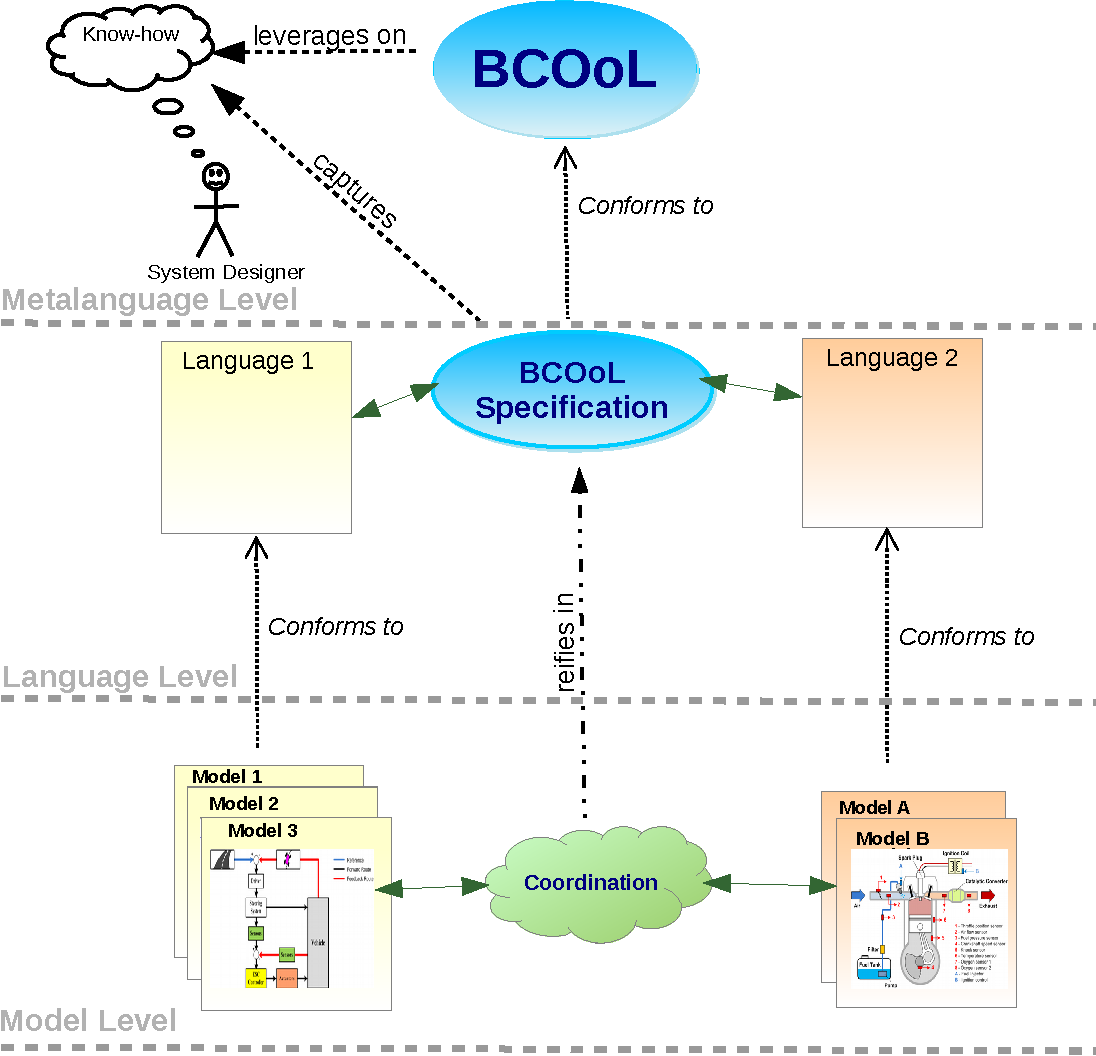
\includegraphics[width=0.7\textwidth]{background/figs/bcoolapp}
%\caption{Overview of Our Approach}
%\label{fig:bcoolapp}
%\end{center}
%\end{figure}	


%\begin{landscape}% Landscape page
%\begin{table}[]
	%\centering
	%\caption{Overview of Behavioral Composition/Coordination Approaches}
	%\label{tbl:overview}
	%\resizebox{\textwidth}{!}{%
		%\begin{tabular}{@{}|c|l|l|c|c|c|c|c|c|c|
			%	>{\columncolor[HTML]{9AFF99}}c |@{}}
			%\toprule
			%\multicolumn{3}{|c|}{} & \multicolumn{2}{c|}{Behavioral Composition Approaches} & \multicolumn{3}{c|}{Coordination %of Model Approaches} & \multicolumn{2}{c|}{Coordination Pattern Approaches} & Our Approach \\ \cmidrule(l){4-11} 
			%\multicolumn{3}{|c|}{\multirow{-2}{*}{}} & Semantic Anchoring & \cite{compostatechartsbib} & Esper & Rapide & BIP & %Ptolemy & Di Natale et. al & BCOoL \\ \midrule
			%\multicolumn{3}{|c|}{Number of Languages/Models Supported} & 1 & 1 & N & N & 1 & Predefined set & 2 & N Languages %\\ \midrule
			%\multicolumn{3}{|c|}{Specification of the Coordination (from a system designer point of view)} &  & Implicit & %Explicit & Explicit & Explicit & Implicit & Impicit & Explicit \\ \midrule
			%\multicolumn{3}{|c|}{Glue (coordination at model level)} &  &  & Formal & Formal & Formal & Java (generated) & C++ %(generated) & Formal (generated) \\ \bottomrule
%		\end{tabular}
%	}
%\end{table}
%\end{landscape}
